\chapter{Introduction}
\label{sec:introduction}

Das Sammeln und Auswerten von Nutzerdaten auf mobilen Endgeräten auch unter „Deep App Tracking“ bekannt sind für viele Anwendungsbereiche unausweichlich. Die Daten wie Nutzerkontext, -aktivität und -status, müssen zunächst aufwendig gesammelt und für den Anwendungsfall aufbereitet werden. Die Auswertung ist zeitaufwändig, spezifisch, und verbraucht viel Ressourcen wie Speicher und Rechenkapazität. Die sensitiven Daten verraten teilweise zu viel über den Nutzer und greifen potenziell dessen Privatsphäre ein. Außerdem ist keine Verknüpfung der Daten gegeben, wodurch man Zusammenhänge, Eigenschaften und Ähnlichkeiten erkennen könnte.
Es wäre sinnvoll, die Komplexität des Nutzerkontexts und Nutzerinteraktionen zu verringern, z.B. indem man sie als Vektoren abbildet, um sie dann je nach Bedarf abzufragen und zu verarbeiten. Diese verteilte Repräsentation hat viele Einsatzzwecke: beispielsweise können damit Ähnlichkeiten von Apps oder Fehler beim Testen der App-Inhalte gefunden werden. Auch kann das Nutzerverhalten Muster in der Mensch-Maschine-Interaktion besser erkannt oder gegebenenfalls gewisse Vorhersagen über zukünftige Aktionen des Nutzers getroffen werden. 
Das Verfahren bietet einen einheitlichen, schnellen und zugleich datenschutzrechtlich unbedenklichen Zugriff auf komprimierte UI-Textelemente und Nutzeraktionen. Derzeit gibt es noch kein vergleichbares Konzept, was auf den Android Accessibility Service spezialisiert wurde und den Doc2Vec Algorithmus als Grundlage verwendet, um die Komplexität des Android UI Trees zu verringern.
Ziel ist es ein Modell zu generieren, was möglichst viele Tree-Daten auf Basis des Android-Accessibility-Services repräsentiert. Diese sollen zunächst zum einen nach textlichem Inhalt eines Screens bzw. dessen Kategorie gefiltert werden können (\ref{fig:encode-decode}). Das beinhaltet konkret z.B. den App-Namen, Textgröße, ggf. die Objekt-Klasse und vor allem den Textinhalt verschiedener Elemente des UI-Trees. Oder zum anderen soll nach der Nutzeraktion gefiltert werden können: z.B. Aktion, Buttonname, Auswahl und Fokus. Zudem könnte noch nach weiteren Features gefiltert werden, wie dem Nutzer-Kontext, Sensorik, Reaktionszeiten, Verweildauer, etc. Gleichzeitig soll die Komplexität der Ausgabe konfigurierbar sein, wobei dies nur den textlichen Inhalt betrifft. Das bedeutet, dass bei einer höheren Komplexitätsstufe ein vergleichbar größerer oder sogar der ganze Inhalt wiedergegeben wird, wobei bei der kleinsten Komplexitätsstufe nur eine einzige Kategorie ausgegeben werden soll.

\begin{figure}[htbp!]
  \centering
  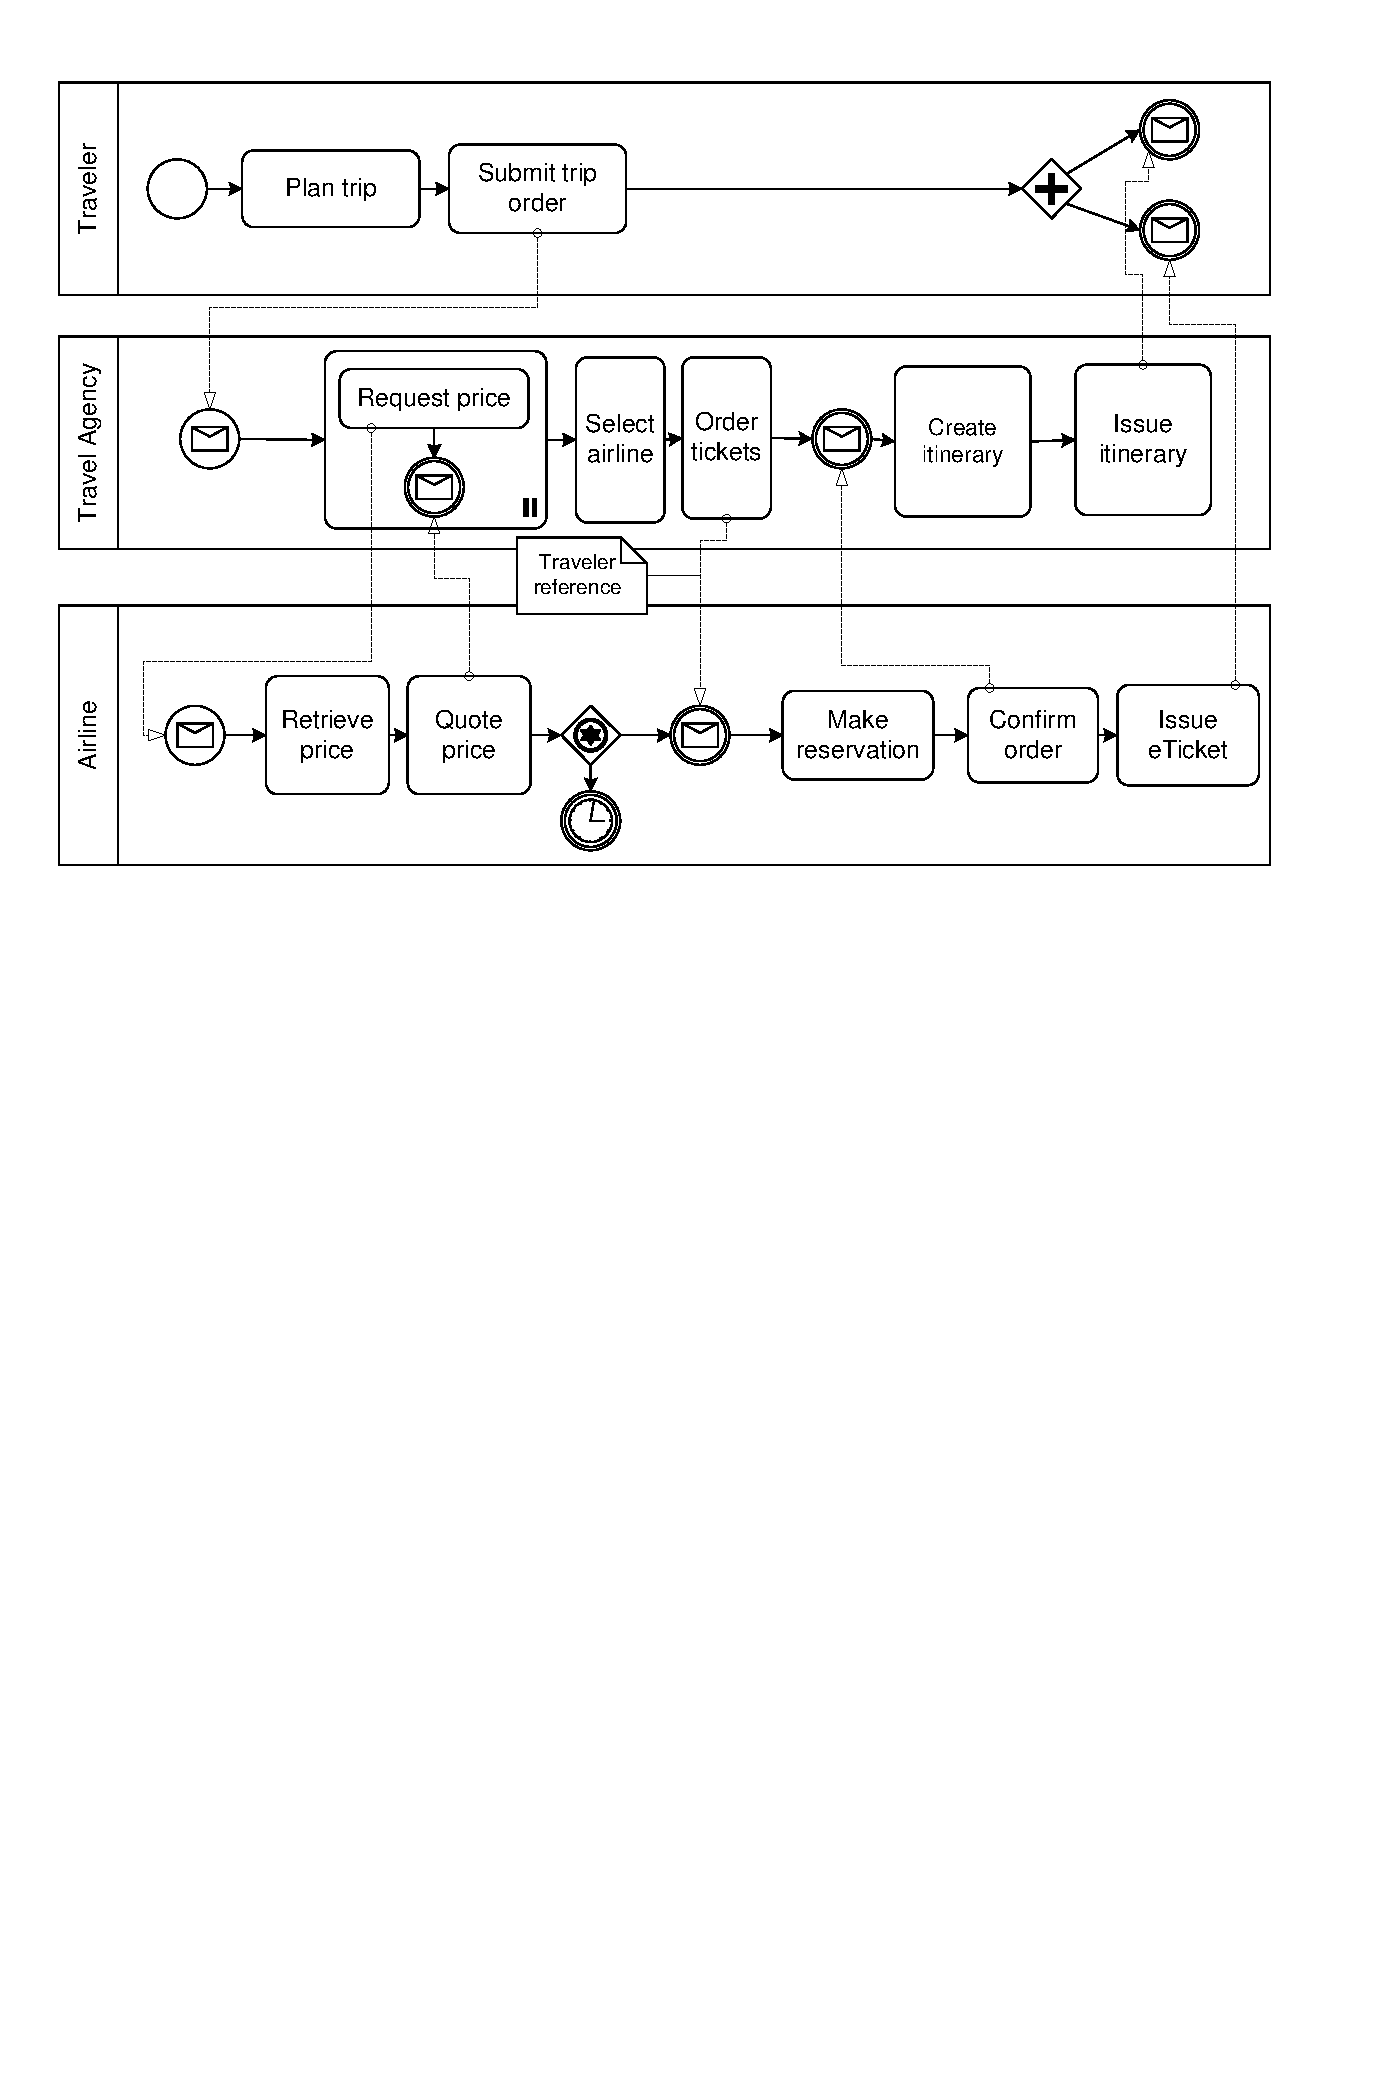
\includegraphics[width=\textwidth]{choreography.pdf}
  \caption{Possible features which can be retrieved by transforming Android Tree Data into a vector representation. Screen-Content (weighted text vectors) can be separated in a single or multiple categories, but validation can be possible on sentimental labeled data, while title and paragraph comparisons are not objectively comparable. A user action could be represented as a category or a more descriptive user intent}
  \label{fig:encode-decode}
\end{figure}

Für die Validierung der Screen-Kategorie können die 32 Play-Store App-Kategorien herangezogen werden \cite{google2023appCategory}. Für die Überprüfung von Nutzeraktionen könnte ein gelabelter Datensatz herangezogen werden, der z.B. folgende Labels enthält: Suche, Texteditierung, Bestätigung, Menü, Zurück, Zoom, Gesture, Scroll, Focus, usw.
Als Grundlage für die textbasierte Einordnung soll das neuronale Netz „Doc2Vec“ \cite{wu2022distributed} dienen. Dieses kann im Gegensatz zur „Bag-of-Words“, oder der „Word2Vec“-Repräsentation auf variablen Textlängen arbeiten und berücksichtigt auch die Reihenfolge der Wörter. „Html2Vec“ spezialisiert sich auf die Verarbeitung von HTML trees und arbeitet mit Gewichtungen abhängig von den HTML-Tags, um die Webseiten bestmöglich zu klassifizieren \cite{wu2022distributed}. Dieses Verfahren könnte neben Activity2Vec \cite{ghods2019activity2vec}, dem TextOnly Modell in Screen2Vec \cite{li2021screen2vec} und Intention2Text \cite{yu2020understanding} als Inspiration für eine optimierte Distributed Representation für Android UI Tree Daten herangezogen werden.
Zur Entwicklung des „AndroidTree2Vec“ Algorithmus, kann das in Python geschriebene Doc2Vec Modell von Gensim \cite{rare2023gensim} erweitert werden. Die Accessibility-Daten werden zunächst über einen eigenen App-Service (Kotlin) zusammengetragen werden. Oder die View Hierarchy könnte aber auch dem Datensatz Rico \cite{deka2017rico} entnommen werden. Wie sich die hierarchischen Daten von bisherigen Datensätzen (wie Rico und ERICA \cite{deka2016erica} mit eigenen Verfahren oder Android UiAutomator-Service \cite{google2023uiAutomator} zu den des Accessibility-Services unterscheiden, muss noch evaluiert werden. 
Es sind bereits ähnliche Modelle wie Screen2Vec \cite{li2021screen2vec} publiziert worden. Eine Verbesserung der dortigen Ergebnisse ist aufgrund des Umfangs der Masterarbeit nicht garantiert.
